%
% File: chap02.tex section 2.2 
% Author: Hongliang Zhong
%
\let\textcircled=\pgftextcircled
\section{The strategy of trade-off}
\label{sec:tradeoff}

The synopsis of Bandit problems have been introduced in Section~\ref{sec:environment}. From this synopsis, we get the difficult point of Bandit problem is to keep a balance between Exploration and Exploitation. So that, it becomes very important to trade off between to exploit from the past knowledge to focus on the arms that seems to yield the highest rewards and to explore further the other arms to identify that better which may be the actual global optimal. 

The easiest way to solve this problem, is to select randomly. However, this way mainly relies on luck. So it is not reliable. Another simple way is called ``Naive Sampling'' approach. At early times, it samples each arm by same number, and then measure the results on comparing these samples. After that, an optimal empirical solution has been shown. But this approach also has a problem, that is, if the initial number of samples is too small, the confidence will be low; if the initial number are huge enough, will waste the cost. Therefore, in this section, we will introduce some effective strategies to solve bandit problems.
\
\
\
\
\
\


%=======

\subsection{Thompson Sampling}
\label{subsec:thompson}

Thompson Sampling \cite{thompson1933likelihood}, a randomized algorithm based on Bayesian ideas, is one of oldest heuristic principle  for Bandit problems. Recently, it has been considered having better empirical performance compared to the state-of-the-art methods after several studies demonstrated \cite{chapelle2011empirical,agrawal2011analysis,agrawal2012thompson}.

The origins of Thompson Sampling has been introduced in Chapter~\ref{chap:introduction}, is from the procedure's inventor  William R. Thompson. Thompson was interested in the general problem of research planning. He was concerned with being able to utilize a small numbers of observations in order to steer actions taken before more data could be collected.
This was in the context of a perceived objection to argument based on small numbers of observations at the time. Thompson posed his problem in terms of deciding between two treatments in a clinical trial. One of the treatments would  be administered to a patient in the trials population and the effect could be observed. These observations could then be incorporated into the decision-making process to improve the odds of the most effective treatment being administered to further patients.

For Bandit problems, this randomized strategy will choose an arm with some probability which matches the probability that the arm is in fact the optimal arm, by giving all past observations of all arm pulls. More reasonable for this randomized chosen is to define the probability that an arm is the best is a Bayesian estimate. 

Being more precise, let $\theta$  be a parameter vector on behavior of a bandit problem. The probability that an arm $k$ is optimal, 
\begin{equation}
P(K=k^{\ast}) = \int_{\theta}\mathds{1}(K=k^{\ast}|\theta)P(\theta)\mathrm{d}\theta.
\end{equation}

An arm is thus pulled with the probability $P(K=k^{\ast})$. This Sampling way could be viewed as forming a decision based on one-step Monte-Carlo Sample by estimating the probability of an arm being the best.

The integral above may not have a closed form solution. The integral may be approximated by quadrature. However, this is undesirable as the running cost of each decision will depend on the difficulty of the multi-armed bandit problem. The insight used in Thompson Sampling is that instead we can sample from a distribution defined by $P(K=k^{\ast})$ by simply first sampling a candidate $\theta$ from the distribution $P(\theta)$. 
Given a candidate $\theta$ we can then just pull the arm that is best given this candidate $(\1(K=k^{\ast}|\theta))$. $P(\theta)$ is initially specified as  a prior and then later inferred using Bayes rule as rewards from arm pulls are observed . The general Thompson Sampling algorithm for a $K$-armed bandit is therefore described as following
%!ALGORITHM-----------------------------
\begin{algo}[Thompson Sampling]
\label{algo:thompson1}
\begin{algorithmic}
\STATE $\ \ $
\STATE Initialise $P_{(\mu_1,\dots,\mu_K)}$, the prior belief of the mean payoffs of arms $1,\dots,K$. 
\STATE Let $H_t$ be the history of action, reward pairs $(r_{\tau}, k_{\tau})$ for $1\leqslant \tau \leqslant t$, $H_1 = \{ \}$
\FOR {each round t = 1,2,\dots, T}
	\STATE Sample $\theta_i,\dots,\theta_K \sim P(\mu_1,\dots,\mu_K|H_t)$.
    \STATE Pull arm $k_t = argmax_{k \in \{1,\dots,K\}} \theta_k$
    \STATE Receive reward $\mathds{1}_{r(k_t)=1}$
	\STATE Let $H_{t+1} = H_t \cup (k_t,\mathds{1}_{r(k_t)=1})$.
\ENDFOR
\end{algorithmic}
\end{algo}
%!----------------------------------------


\textbf{Optimism in Thompson Sampling}
There is a question, what is the tradeoff between exploration and exploitation for Thompson Sampling. May \cite{may2012optimistic} tried to separate the two aspects of this algorithm. To do this, he defined the exploitative value of an arm to be the expected payoff of an arm conditioned on the rewards. The estimated value of an arm could be seen as the value of the sampling drawn from the posterioi distribution for the arm. With these, the exploratory value of an arm could then by found by subtracting the exploitative value from the estimated sample value. They observed that this exploratory value could sometimes be negative and so there would be no value from an exploration point of view to pull the arm. The exploratory value of an arm is only negative when the sample estimate drawn from the posterior is less than the exploitative value of the arm. 

In Thompson Sampling, samples are drawn from the posterior distribution of each arm, that is $\theta_k(t)\sim P_{(\mu_k)}$. Instead, Optimistic Thompson Sampling drawn samples such that $\theta_k(t) = max(\mathbb{E}[\mu_k],s_k(t))$ where $s_k(t)\sim P_{(\mu_k)}$. In other words if a sample from the posterior distributions is less than the mean of the distribution, then we take the sample to be then mean. This ensures that the exploratory value of an action is always positive. In Appendix Algorithm~\ref{algo:thompson3} more formally presents the algorithm specifically for the Bernoulli bandit. May\cite{may2012optimistic} observed empirically that Optimistic Thompson Sampling performed better than standard Thompson Sampling.(See in Appendix~\ref{algo:thompson3})

\subsection{Boltzmann Exploration (Softmax)}
\label{subsec:softmax}
This section, is about  Boltzmann Exploration (also named  Softmax), which is based on the axiom of choice \cite{luce1959individual} and pick each arm with a probability that is proportional to its average  behavior. Arms with greater empirical means could be therefore picked with higher probability. Softmax  selects arms by using a Boltzmann distribution. Given initial empirical means $\hat{\mu}_1(0),\dots,\hat{\mu}_K(0)$,
\begin{equation}
\label{equa:boltzmann}
p_k(t+1) = \frac{\exp{\hat{\mu}_k(t)/\tau}}{\sum_{i=1}^{K}\exp{\hat{\mu}_i(t)/\tau}}, \text{where } k\in \{1,\dots,K\}
\end{equation}

Softmax may depend on the task and on human factors by the only parameter $\tau$. Where $\tau$ is a temperature parameter, controlling the randomness of the choice. When $\tau = 0$, Boltzmann Exploration acts like pure greedy. On contrast, $\tau$ tends to infinity, the algorithms picks arms uniformly at random. Most people find it easier to set the $\tau$ requires knowledge of the likely action values and of powers of $e$.

%!ALGORITHM-----------------------------
%!--------------------------------------
\begin{algo}[SoftMax]
%\caption{SoftMax}
\label{algo:softmax1}
\begin{algorithmic}
\STATE {\ }
\STATE Parameter: real number $\tau > 0$
\STATE Initialization: Set $\hat{\mu}_k(0) = 0$ for $\forall k \in [1,\dots,K]$
\FOR {each round t = 1,2,\dots, T}
	\STATE Sample arms $i$ according to the distribution $P(t)$, where
    \[P_k(t) = \frac{\exp \left(\hat{\mu}_k(t-1)/\tau\right)}{\sum_{i=1}^{K} \exp \left(\hat{\mu}_i(t-1)/\tau\right)}\]
    \STATE Receive the reward $r_{k_t}$, here $k_t$ is the sampled arm for instant t 
    \STATE Let $\hat{\mu}_{k}(t) = \sum_t r_{k,t}/ \sum_t \1_{k = k_t,t}$
\ENDFOR
\end{algorithmic}
\end{algo}
%!----------------------------------------

The Softmax strategy could be modified in the same way as the $\epsilon$-greedy strategy in Section~\ref{subsec:greedy} into decreasing Softmax where the temperature decreases with the number of rounds played. The decreasing Softmax is identical to the Softmax but with a temperature $\tau_t = \tau_0/t$ that depends on the index $t$ of the current round. The choice of the value of $\tau_0$ is left to the user. The decreasing Softmax is analyzed by Cesa-Bianchi \cite{cesa1998finite} with the Softmix algorithm. 

A more complicated variant of the Softmax algorithm, the EXP3 ``(see in Appendix~\ref{algo:softmax2})exponential weight algorithm for Exploration/Exploitation'' is introduced in \cite{auer1995gambling}. The probability of choosing the arm $k$ at the round of index $t$ is defined by 
\begin{equation}
P_k(t) = (1-\gamma)\frac{w_k(t)}{\sum_{i=1}^{K}w_i(t)}+\frac{\gamma}{K}
\end{equation}
where $w_i(t+1) = w_i(t) exp\left(\gamma\frac{r_i(t)}{P_i(t)K}\right)$,
if the arm $i$ has been pulled at time t with $r_i(t)$ being the observed reward,
$w_i(t+1) = w_i(t)$ otherwise. The choice of the value of the parameter $\gamma\in (0,1]$ is left to the user.
The main idea is to divide the actual gain $r_i(t)$ by the probability $P_i(t)$ that the action was chosen. For a modified version of EXP3, with $\gamma$ decreasing over time, it is shown by \cite{auer2003nonstochastic}, that a regret of $O(\sqrt{KT\log{K}})$ is achieved.

\subsection{Upper Confidence Bound}
\label{subsec:ucb}
Upper Confidence Bound (UCB) was proposed by Lai \cite{lai1985asymptotically}, to deal with the Exploration and Exploitation dilemma in the Multi-Armed Bandit problem by using Upper Confidence Values. Most strategy for trading off Exploration and Exploitation, they have one weakness: they do not keep track of how much they know about any of options available to them. They pay much more attention only to how much reward they got. This means that they will under-explore options whose initial experiences were not rewarding, even though they don't have enough data to be confident about those options. But UCB can do better that pays attention to not only what it knows, but also how much it knows. 

For example, in stochastic Multi-Armed Bandit problem, gambler has to choose in trials $t\in \{1,2,\dots,T\}$ an arm from a given set of arms $\mathscr{K} = \{1,\dots,K\}$. 
In each trial $t$ the gambler obtains random reward $r_{k,t}\in \{0,1\}$ for choosing arm $k$. 
It is assumed that for each arm $k$ the random reward $r_{k,t}$ is independent and identically distributed random variables with mean $\mu_k$ which is unknown. 
Further, it is assumed that the rewards $r_{k,t}$ and $r_{k',t'}$ for distinct arms $k,k'$ are independent for all $k\neq k' \in \mathscr{K}$ and all $t, t' \in \mathscr{T}$.
 
The gambler's aim is to compete with the arm giving highest mean reward $\mu^{\ast}:= max_{k\in \mathscr{K}} \mu_k$. The arm with the best estimate $\hat{\mu}^{\ast}$ so far serves as a creteria, and other arms are played only if the upper bound of a suitable confidence interval is at least $\hat{\mu}^{\ast}$. That way, within $T$ trials each suboptimal arm can be shown to be played at most $\left(\frac{1}{D_{KL}}+o(1)\right)\log{T}$ times in expectation, where $D_{KL}$ measures the distance between the reward distributions of the optimal and the suboptimal arm by the Kellback-Leibler divergence, and $o(1) \rightarrow 0$ as $T \rightarrow \infty$. This bound was also shown to be asymptotically optimal\cite{lai1985asymptotically}.

Auer \cite{auer2003using} introduced the simple, yet efficient UCB algorithm, that is also based on the ideas of Lai's. After playing each arm once for initialization, UCB chooses at trial $t$ the arm $k$ that maximizes
\begin{equation}
\label{equa:UCB}
\hat{\mu}_k+\sqrt{\frac{2\log{t}}{n_k}}
\end{equation},
where $\hat{\mu}_k$ is the average reward obtained from arm $k$, and $n_k$ is the number of times arm $k$ has been played up to trial $t$. The value in Equation~\ref{equa:UCB} can be interpreted as the Upper Bound of a confidence interval, so that the true mean reward of each arm $k$ with high probability is below this upper confidence bound.

In particular, the upper confidence value of the optimal arm will be higher than the true optimal mean reward $\mu^{\ast}$ with high probability. Consequently, as soon as a suboptimal arm $k$ has been played sufficiently often so that the length of the confidence interval $\sqrt{\frac{2\log{t}}{n_k}}$ is small enough to guarantee that
\[\hat{\mu}_k+\sqrt{\frac{2\log{t}}{n_k}} < \mu^{\ast}
\],
arm $k$ will not be played anymore with high probability. As it also holds that with high probability
\[\hat{\mu}_k<\mu_k+\sqrt{\frac{2\log{t}}{n_k}}\],
arm $k$ is not played as soon as 
\[2\sqrt{\frac{2\log{t}}{n_k}}<\mu^{\ast}-\mu_k\],
that is, as soon as arm $k$ has been played
\[\left \lceil \frac{8\log{t}}{(r^{\ast}-r_k)^2} \right \rceil\]
times. This informal argument can be made stringent to show that each suboptimal arm $k$ in expectation will not be played more often than $\frac{\log{T}}{\Delta_k^2}$ times within $T$ trials, 
where $\Delta_k:=\mu^{\ast}-\mu_k$ is the distance between the optimal mean reward and $\mu_k$.

%!ALGORITHM-----------------------------
%!--------------------------------------
\begin{algo}[Improved UCB algorithm]
%\caption{Improved UCB algorithm}
\label{algo:UCB1}
\begin{algorithmic}
\STATE {\ }
\STATE Set arms $\mathscr{K}= \{1,\dots,K\}$, all playing times $\mathscr{T} = 1,2, \dots, T$
\STATE Initialization: Set $\tilde{\Delta}_0:=1$, and $B_0:=\mathscr{K}$.
\FOR {each round $t = 1,2,\dots, \left \lfloor \frac{1}{2}\log{\frac{T}{e}} \right \rfloor$ }
	\STATE Select arm: if $|B_m|>1$, choose each arm in $B_m$ until the total number of times it has been chosen is $n_m:= \left \lceil \frac{2\log{T\tilde{\Delta}^2_m}}{\tilde{\Delta}^2_m} \right \rceil$. Otherwise choose the single $B_m$ until step $T$ is reached.
	\STATE Eliminate arm: Delete all arms $i$ from $B_m$ for which
    \[ \left\{ \hat{\mu}_i+\sqrt{\frac{\log{T\tilde{\Delta}^2_m}}{2n_m}} \right\} < \text{max}_{j\in B} \left\{ \hat{\mu}_j - \sqrt{\frac{\log{T\tilde{\Delta}^2_m}}{2n_m}}\right\} \] in order to obtain $B_{m+1}$. Here $\hat{\mu}_j$ is the average reward obtained from arm $j$.
    \STATE	Reset $\tilde{\Delta}_m$: Set $\tilde{\Delta}_{m+1} = \frac{\tilde{\Delta}_m}{2}$
\ENDFOR
\end{algorithmic}
\end{algo}
%!----------------------------------------

In \cite{auer2010ucb}, Auer proposed an improved UCB algorithm (shown in Algorithm~\ref{algo:UCB1}). In this improved model, gambler can access to the values $\Delta_k$, one could directly modify the confidence intervals of UCB as given \cite{agrawal1995sample} to $\sqrt{\frac{2\log{t\Delta_k^2}}{n_k}}$, and the proof of the claimed regret bound would be straightforward.

However, since the $\Delta_k$ is unknown to the learner, the modified algorithm shown in Algorithm~\ref{algo:UCB1} guesses the values $\Delta_k$ by a value $\tilde{\Delta}$, which is initialized to 1 and halved each time the confidence intervals become shorter than $\tilde{\Delta}$. Note that compared to the original UCB algorithm the confidence intervals are shorter, in particular for arms with high estimated reward. Unlike the original UCB algorithm, our modification eliminates arms that perform bad. As the analysis will show, each suboptimal arm is eliminated as soon as $\tilde{\Delta}<\frac{\Delta_k}{2}$, provided that the confidence intervals hold. Similar arm elimination algorithms were already proposed in \cite{even2006action}. 

\subsection{Epsilon-Greedy}
\label{subsec:greedy}

In this section, we are going to introduce a simple algorithm for trading off exploration and exploitation. This strategy is called $\epsilon$-Greedy\cite{Sutton98} (shown in Appendix~\ref{algo:epsilon}). In computer science, a greedy algorithm is an algorithm that always takes whatever action seems best at the present moment, even when that decision might lead to bad long term consequences. The $\epsilon$-greedy algorithm is almost a greedy algorithm because it generally exploits the best available option, but also have some chance to explore the other available options. 
\begin{figure}[!h]
\centering{
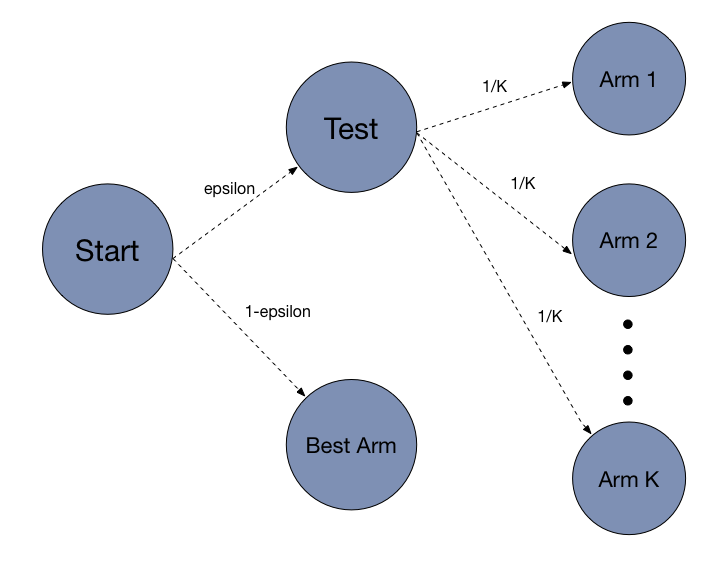
\includegraphics[scale = 0.4]{chapters/chapter02/fig02/epsilongreedy.png}}
\caption{the mechanism of epsilon-greedy}
\label{fig:epsilon}
\end{figure}

Let's be more concrete to the mechanism of $\epsilon$-greedy algorithm. It works by randomly oscillating between the purely randomized experimentation and instinct to maximize profits. The $\epsilon$-greedy is one of the easiest bandit algorithms to understand because it tries to be fair to the two opposite goals of exploration and exploitation by using a mechanism (see the Figure~\ref{fig:epsilon}). Take a simple example to understand easily: it is just like flipping a coin. If you flip a coin and it comes up heads, you should explore for a moment. But if the coin comes up tails, you should exploit.

The formal process as follows,
\begin{itemize}
\item Firstly, pick a parameter $\epsilon \in [0,1]$, 
\item Then, at each step greedily play the object with highest empirical mean reward with probability $1-\epsilon$ and play a random arm with probability $\epsilon$. 
\item Receives the reward from the arm chosen
\item Finally, update the empirical means of each arm.
\end{itemize}

%!ALGORITHM-----------------------------
%!--------------------------------------
\begin{algo}[$\epsilon$-Greedy]
%\caption{$\epsilon$-Greedy}
\label{algo:epsilon}
\begin{algorithmic}
\STATE {\ }
\STATE Initialise $P_{(\mu_1,\dots,\mu_K)}$, the prior belif of the mean payoffs of arms $1,\dots,K$. 
\FOR {each round t = 1,2,\dots, T}
	\STATE Pull arm $k_t = \begin{cases}
    \text{argmax}_{k\in \{1,\dots,K\}} P_{(\mu_k)} & \text{with probability}\ \epsilon \\
    \text{select randomly} & \text{with probability}\ 1-\epsilon
    \end{cases}$ 
    \STATE Receive reward $r_{(k_t)}$
	\STATE Update $\mu_{k_t}$ by the reward $r_{(k_t)}$.
\ENDFOR
\end{algorithmic}
\end{algo}
%!----------------------------------------

Auer~\cite{Auer02Finite} has proven that, if $\epsilon$ is allowed to be a certain function $\epsilon_t$ following the current time step $t$, namely $\epsilon_t = K/(d^2t)$, then the regret grows logarithmically like $(K \log{T}/d^2)$, provided $d$ less than the number of objects with minimum regret . While this bound has a suboptimal dependence on $d$. In Auer's~\cite{Auer02Finite} same paper, it show that this algorithm performs well in practice, but the performance degrades quickly if $d$ is not chosen as a tight lower bound.

Compared to other more complex methods, $\epsilon$-greedy is often hard to beat and reported to be often the method of the first choice as stated . In practice, however, a drawback of $\epsilon$-greedy is that it is unclear which setting of $\epsilon$ leads to good results for a given learning problem. For this reason, the experimenter has to rigorously hand tune $\epsilon$ for obtaining good results, which can be a very time-consuming task in practice depending on the complexity of the target application.

One method that aims at overcoming the above mentioned limitation of $\epsilon$-greedy is ``Value-Difference Based Exploration''(VDBE)\cite{tokic2010adaptive}. In contrast to pure $\epsilon$-greedy, VDBE adapts a state-dependent exploration-probability. The basic idea of VDBE is to extend the $\epsilon$-greedy method by controlling a state-dependent exploration probability, $\epsilon(s)$, in dependence of the value-function error instead of manual tuning. The desired behavior is to have the agent more explorative in situations when the knowledge about the environment is uncertain, i.e. at the beginning of the learning process, which is recognized as large changes in the value function. On the other hand, the exploration rate should be reduced as the agent's knowledge becomes certain about the environment, which can be recognized as very small or no changes in the value function. 
